%
% flaeche.tex
%
% (c) 2021 Prof Dr Andreas Müller, OST Ostschweizer Fachhochschule
%
\section{Flächeninhalt
\label{buch:geometrie:section:flaeche}}
\rhead{Flächeninhalt}
Die elementare Definition des Integrals versucht, den Flächeninhalt
unter dem Graphen der Funktion $y=f(x)$ zu definieren.
Die Erfahrung zeigt, dass es nicht immer einfach ist, ein Integral in
geschlossener Form zu berechnen.
Solche Integrale können auf sinnvolle neue spezielle Funktionen führen.

\subsection{Berechnung des Flächeninhaltes in kartesischen Koordinaten}
Wir betrachten in diesem Abschnitt nur die Berechnung des
Flächeninhaltes von Teilgebieten der Ebene $\mathbb{R}^2$
aus ihrer Berandung.
Sei $\gamma\colon I \to\mathbb{R}^2$ eine Kurve und 
\[
a=t_0<t_1<t_2<\dots t_{n-2}<t_{n-1}<t_n=b
\]
eine Unterteilung des Intervalls.
Die Kurve muss ausserdem geschlossen sein, also $\gamma(a)=\gamma(b)$.
Die Punkte $\gamma(t_i)$ sind die Ecken eines Polygons, das die gesucht
Fläche approximiert.

Der Flächeninhalt des Polygons kann mit der Schuhbändelformel
\cite[p.~184]{buch:linalg}
berechnet werden.

\begin{align*}
F
&=
\sum_{i=0}^{n-1}
\frac12
\biggl|\begin{matrix}
x(t_i)    &y(t_i)    \\
x(t_{i+1})&y(t_{i+1})
\end{matrix}\biggr|
\approx
\frac12
\sum_{i=0}^{n-1}
\biggl|\begin{matrix}
x(t_i)    &y(t_i)    \\
x(t_{i+1})-x(t_i)&y(t_{i+1})-y(t_i)
\end{matrix}\biggr|
\\
&=
\frac12
\sum_{i=0}^{n-1}
\biggl|\begin{matrix}
x(t_i)                        &y(t_i)    \\
\dot{x}(t_{i+1}) (t_{i+1}-t_i)& \dot{y}(t_{i+1}) (t_{i+1}-t_i)
\end{matrix}\biggr|
\\
&=
\frac12
\sum_{i=0}^{n-1}
\biggl|\begin{matrix}
x(t_i)           &y(t_i)    \\
\dot{x}(t_{i+1}) & \dot{y}(t_{i+1})
\end{matrix}\biggr|
(t_{i+1}-t_{i}).
\end{align*}
Die letzte Summe kann als Riemann-Summe und damit als Approximation für
das Integral
\[
F
\approx
\frac12
\int_a^b
\left|\begin{pmatrix} x(t)&y(t)\\\dot{x}(t)&\dot{y}(t)\end{pmatrix}\right|
\,dt
\]
gesehen werden.
Der Flächeninhalt des Gebietes, welches von der Kurve $\gamma$
berandet wird, ist daher
\begin{equation}
F
=
\frac12
\int_a^b x(t)\dot{y}(t)-y(t)\dot{x}(t)\,dt.
\label{buch:geometrie:eqn:flaeche}
\end{equation}

Die Formel~\eqref{buch:geometrie:eqn:flaeche} gilt auch für nicht
geschlossene Kurven.
Sie berechnet dann den Flächeninhalt eines Gebietes, welches von
der Strecke vom Ursprung zu $\gamma(a)$, der Kurve von $\gamma(a)$ nach
$\gamma(b)$ und von der Strecke von $\gamma(b)$ zurück zum Nullpunkt
berandet wird.

\begin{beispiel}
Der Flächeninhalt eines Kreissektors mit Öffnungswinkel $\alpha$ ist
kann mit Hilfe der Parametrisierung
\[
\gamma
\colon
[0,\alpha] \to \mathbb{R}^2
:
t\mapsto \begin{pmatrix}r\cos t\\ r\sin t\end{pmatrix}
\]
berechnet werden.
Das Integral~\eqref{buch:geometrie:eqn:flaeche} wird dann zu
\begin{align*}
F
&=
\frac12
\int_0^\alpha r\cos t \cdot r\cos t - r\sin t \cdot (-r\sin t)\,dt
\\
&=
\frac{r^2}2
\int_0^\alpha
\cos^2t + \sin^2t\,dt
=
\frac{r^2\alpha}2,
\end{align*}
wie erwartet.
\end{beispiel}

\subsubsection{Flächeninhalt in Polarkoordinaten}
Ist die Kurve in Polarkoordinaten durch die Funktion
$\varphi\mapsto r(\varphi)$ gegeben, dann kann man $\varphi$ als
Parameter verwenden.
Die Determinante in der Flächenformel wird
\begin{align*}
\biggl|
\begin{matrix}
x(t_i)& y(t_i)\\
\dot{x}(t_i)& \dot{y}(t_i)
\end{matrix}
\biggr|
&=
\biggl|
\begin{matrix}
r(\varphi)\cos\varphi&r(\varphi)\sin\varphi\\
-r(\varphi)\sin\varphi+r'(\varphi)\cos\varphi
	&r(\varphi)\cos\varphi+r'(\varphi)\sin\varphi
\end{matrix}
\biggr|.
\end{align*}
Der Integrand in der Flächenformel wird dann
\[
\frac12\bigl(
r(\varphi)^2 \cos^2\varphi +r(\varphi)r'(\varphi)\cos\varphi\sin\varphi
+
r(\varphi)^2 \sin^2\varphi -r(\varphi)r'(\varphi)\sin\varphi\cos\varphi
\bigr)
=
\frac{r(\varphi)^2}2
\]
und die Fläche kann mit
\[
F(\alpha,\beta)=\int_\alpha^\beta \frac{r(\varphi)^2}{2}\,d\varphi
\]
berechnet werden.

\subsection{Flächeninhalt von Ellipsen und Hyperbeln}
Ellipsen und Hyperbeln sind besonders einfach zu parametrisieren und
damit ist auch die Fläche, die von Ellipsen oder Hyperbeln berandet
wird, besonders einfach zu berechnen.
Der Flächeninhalt eines Ellipsensektors hat eine besondere Bedeutung
für die Formulierung der Keplerschen Gesetze der Planetenbewegung.

\subsubsection{Ellipse}
Für die Ellipse mit der Gleichung
\[
\frac{x^2}{a^2}+\frac{y^2}{b^2}=1
\]
kann man mit der Parametrisierung
\[
\gamma\colon
[0,2\pi] \to \mathbb{R}^2
:
t \mapsto \begin{pmatrix}a\cos t\\ b\sin t\end{pmatrix}
\]
beschreiben.
Einen Sektor zwischen den Winkeln $\alpha$ und $\beta$
\begin{align*}
F
&=
\int_\alpha^\beta a\cos t \cdot b\cos t-b\sin t\cdot (-a\sin t)\,dt
\\
&=
ab
\int_\alpha^\beta \cos^2 t + \sin^2 t\,dt
=ab(\beta-\alpha).
\end{align*}
Dieses Resultat ist auch rein geometrisch leicht nachzuvollziehen:
Der Sektor entsteht dadurch, dass man ein Kreissektor mit Radius $a$
entlang der $y$-Achse um den Faktor $b/a$ gestaucht wird.
Aus dem Flächeninhalt $a^2(\beta-\alpha)$ des Kreissektors wird dann
der Flächeninhalt $a^2(\beta-\alpha)\cdot \frac{b}{a}=ab(\beta-\alpha)$.

\subsubsection{Hyperbel}
\begin{figure}
\centering
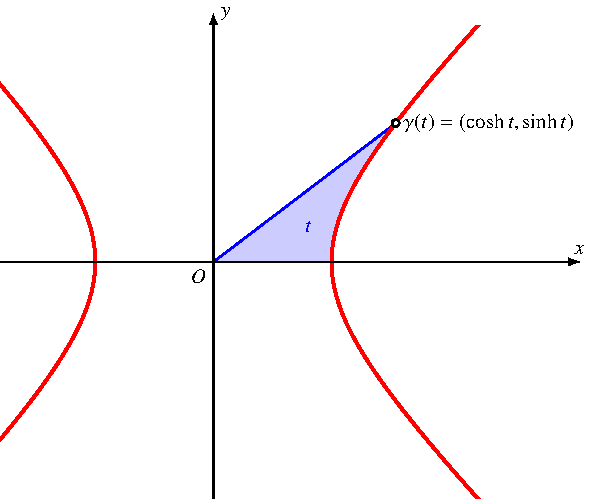
\includegraphics{chapters/030-geometrie/images/hyperbelflaeche.pdf}
\caption{Das Argument $t$ der hyperbolischen Funktionen ist der Inhalt
des krummlinig berandeten Dreiecks, bestehend aus der Strecke 
vom Nullpunkt $O$ zum Punkte $(1,0)$, dem Hyperbelbogen bis zum
Punkt $\gamma(t)=(\cosh t,\sinh t)$ und schliesslich der Strecke
von $\gamma(t)$ zurück zum Nullpunkt.
\label{buch:geometrie:fig:hyperbelflaeche}}
\end{figure}
Die hyperbolischen Funktionen geben eine einfache Parametrisierung
der in Abbildung~\ref{buch:geometrie:fig:hyperbelflaeche}
dargestellten Hyperbel mit der Gleichung
\(
x^2-y^2=1
\).
Der in der Abbildung blau hervorgehobene Flächeninhalt ist der Wert
des Integrals
\begin{align*}
F(t)
&=
\int_0^t
\biggl|
\begin{matrix}
\cosh s&\sinh s\\
\sinh s&\cosh s
\end{matrix}
\biggr|
\,ds
=
\int_0^t
\cosh^2s-\sinh^2s\,ds
=
\int_0^t ds = t.
\end{align*}
Das Argument $t$ der hyperbolischen Funktionen ist also der Flächeninhalt
des von der Hyperbel krummlinig berandeten Dreiecks.
Daher heissen die Umkehrfunktionen der hyperbolischen Funktionen
$\operatorname{arsinh}y$ und $\operatorname{arcosh}y$, Abkürzung
für {\em area cuius sinus hyperbolicus $y$ est}, Fläche, deren zugehöriger
Wert des Sinus hyperbolicus $y$ ist.

\subsubsection{Fokalgleichung in Polarkoordinaten}
\begin{figure}
\centering
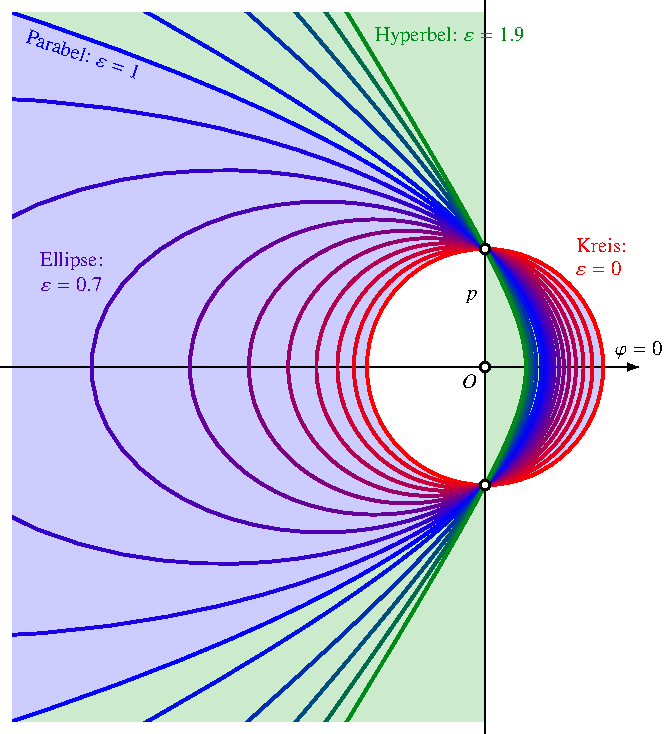
\includegraphics{chapters/030-geometrie/images/polargleichung.pdf}
\caption{Polargleichung der Kegelschnitte mit konstantem Wert für den
Parameter $p$ und verschiedene Werte der Exzentrizität $\varepsilon$.
Der Kreis (rot) hat Exzentrizität $\varepsilon=0$,
die Parabel (blau) hat $\varepsilon=1$.
Für $0<\varepsilon<1$ entstehen Ellipsen, die im blauen Bereich liegen,
für $\varepsilon>1$ entstehen Hyperbeln, die im grün hinterlegten Teil
der Ebene liegen.
\label{buch:geometrie:fig:polargleichung}}
\end{figure}
Das zweite Keplersche Gesetz über Planetenbahnen besagt, dass sich ein
Planet auf seiner elliptischen Bahn um die Sonne so bewegt, dass
sein Radiusvektor in gleichen Zeiten gleiche Flächen überstreicht.
Die bisher verwendete Parametrisierung hat den Mittelpunkt der Ellipse
im Nullpunkt, nach dem ersten Keplerschen Gesetz ist aber müssen
wir eine Parametrisierung verwenden so, dass der Brennpunkt im
Ursprung liegt.
In Polarkoordinaten ist
\begin{equation}
r(\varphi) = \frac{p}{1+\varepsilon \cos\varphi}
\label{buch:geometrie:eqn:polargleichung}
\end{equation}
die sogenannte {\em Polargleichung} für die Kegelschnitte.
Für $\varepsilon=0$ wird $r(\varphi)=p$ konstant, die Gleichung
beschreibt in diesem Fall einen Kreis.
Für $\varepsilon=1$ entsteht eine Parabel.
Werte zwischen $0$ und $1$ parametrisieren Ellipsen mit verschiedener
Exzentrizität, Werte grösser als $1$ führen auf Hyperbeln.
Abbildung~\ref{buch:geometrie:fig:polargleichung} zeigt alle vier Fälle.

Die zwischen den Polarwinkeln $\alpha$ und $\beta$ überstrichene Fläche
wird durch das Integral
\[
F(\alpha,\beta)
=
\int_\alpha^\beta
\frac{r(\varphi)^2}2
\,d\varphi
=
\frac12 \int_\alpha^\beta
\frac{p^2 \,d\varphi}{(1+\varepsilon\cos\varphi)^2}
\]
Das Integral kann in geschlossener Form angegeben werden, die Formeln
sind aber ziemlich kompliziert und für uns hier nicht weiter nützlich.



